\documentclass{standalone}
\usepackage{tikz}
\usetikzlibrary{calc,decorations.pathmorphing}
\begin{document}
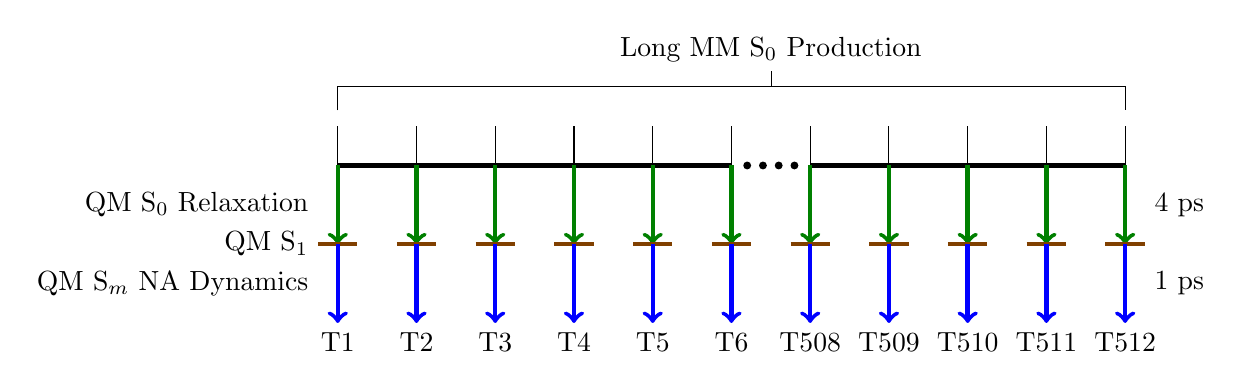
\begin{tikzpicture}
  \draw[ultra thick] (0,0) -- (5,0);
  \foreach \x in {5.2,5.4,...,5.8}{
    \fill (\x,0) circle (0.05);
  }
  \draw[ultra thick] (6,0) -- (10,0);
  \foreach \x in {0,1,...,10}{
    \draw (\x,-0.5) -- (\x,0.5);
    \draw[ultra thick, green!50!black, ->] (\x,0) -- (\x,-1);
    \draw[ultra thick, orange!50!black] (\x-0.25,-1) -- (\x+0.25,-1);
  }
  \foreach \x in {0,1,...,10}{
    \draw[ultra thick, blue, ->] (\x,-1) -- (\x,-2);
  }
  \foreach[count=\i, evaluate=\i as \t using int(\i)] \x in {0,...,5}{
    \node[below] at (\x,-2) {T\t};
  }
  \foreach[count=\i, evaluate=\i as \t using int(\i+507)] \x in {6,...,10}{
    \node[below] at (\x,-2) {T\t};
  }
  \node[left] at (-0.25,-0.5) {QM S$_0$ Relaxation};
  \node[left] at (-0.25,-1) {QM S$_1$};
  \node[left] at (-0.25,-1.5) {QM S$_m$ NA Dynamics};

  \node[right] at (10.25,-0.5) {4 ps};
  \node[right] at (10.25,-1.5) {1 ps};
  \draw[very thin] (0,0.7) -- (0,1) -- (10,1) -- (10,0.7);
  \draw[very thin] (5.5,1) -- (5.5,1.2) node[above] {Long MM S$_0$ Production};
\end{tikzpicture}
\end{document}
